
%\documentclass[mathserif]{beamer}
\documentclass[handout]{beamer}
%\usetheme{Goettingen}
%\usetheme{Warsaw}
\usetheme{Singapore}



%\usetheme{Frankfurt}
%\usetheme{Copenhagen}
%\usetheme{Szeged}
%\usetheme{Montpellier}
%\usetheme{CambridgeUS}
%\usecolortheme{}
%\setbeamercovered{transparent}
\usepackage[english, activeacute]{babel}
\usepackage[utf8]{inputenc}
\usepackage{amsmath, amssymb}
\usepackage{dsfont}
\usepackage{graphics}
\usepackage{cases}
\usepackage{graphicx}
\usepackage{pgf}
\usepackage{epsfig}
\usepackage{amssymb}
\usepackage{multirow}	
\usepackage{amstext}
\usepackage[ruled,vlined,lined]{algorithm2e}
\usepackage{amsmath}
\usepackage{epic}
\usepackage{epsfig}
\usepackage{fontenc}
\usepackage{framed,color}
\usepackage{palatino, url, multicol}
%\algsetup{indent=2em}
\newcommand{\factorial}{\ensuremath{\mbox{\sc Factorial}}}
\newcommand{\BIGOP}[1]{\mathop{\mathchoice%
{\raise-0.22em\hbox{\huge $#1$}}%
{\raise-0.05em\hbox{\Large $#1$}}{\hbox{\large $#1$}}{#1}}}
\newcommand{\bigtimes}{\BIGOP{\times}}
\vspace{-0.5cm}
\title{Natural Language Processing \\ Neural Networks}
\vspace{-0.5cm}
\author[Felipe Bravo Márquez]{\footnotesize
%\author{\footnotesize  
 \textcolor[rgb]{0.00,0.00,1.00}{Felipe Bravo-Marquez}} 
  
 

\date{\today}

\begin{document}
\begin{frame}
\titlepage


\end{frame}





\begin{frame}{Introduction to Neural Networks}
\begin{scriptsize}
\begin{itemize}
\item Very popular machine learning models formed by units called \textbf{neurons}.
\item A neuron is a computational unit that has scalar inputs and outputs. 
\item  Each input has an associated weight $w$.
 \item The neuron multiplies each input by its weight, and then sums them (other functions such as \textbf{max} are also possible). 
\item It applies an activation function $g$ (usually non-linear) to the result, and passes it to its output.
\item Multiple layers can be stacked.
\end{itemize}


\end{scriptsize}
\end{frame}


\begin{frame}{Activation Functions}

\begin{scriptsize}
\begin{itemize}
\item The nonlinear activation function $g$ has a crucial role in the network's ability to represent complex functions. 
\item Without the nonlinearity in g, the neural network can only represent linear transformations of the input.
\end{itemize}


\end{scriptsize}


\end{frame}


\begin{frame}{Feedforward Network with two Layers}


\begin{figure}[htb]
	\centering
	 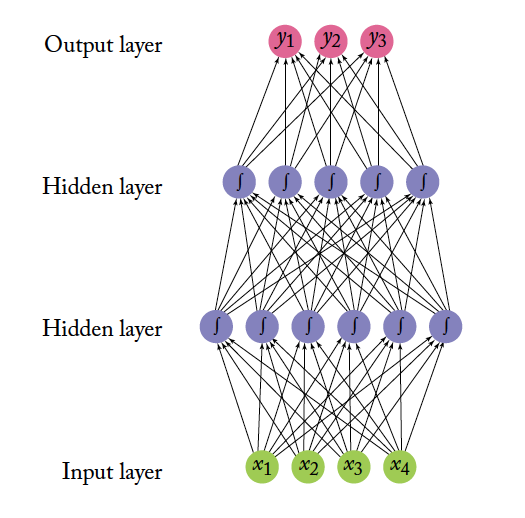
\includegraphics[scale=0.38]{pics/NN-example.png}
\end{figure}

\footnotetext{Source:\cite{goldberg2017neural}}

\end{frame}



\begin{frame}{Feedforward Network Neural Networks}
\begin{scriptsize}
\begin{itemize}
\item The feedforward network from the picture is a stack of linear models separated by nonlinear functions.
\item The values of each row of neurons in the network can be thought of as a vector. 

\item The input layer is a 4-dimensional vector $(\vec{x})$, and the layer above it is a 6-dimensional vector $(\vec{h}^1)$.
\item The fully connected layer can be thought of as a linear transformation from 4 dimensions to 6 dimensions. 
\item A fully connected layer implements a vector-matrix multiplication, $\vec{h}=\vec{x}W$.
\item The weight of the connection from the $i$-th neuron in the input row to the $j$-th neuron in the output row is $W_{[i,j]}$.
\item The values of $\vec{h}$ are transformed by a nonlinear function $g$ that is applied to each value before being passed on as input to the next layer.

\end{itemize}

\footnotetext{Vectors are assumed to be row vectors and superscript indices correspond to network layers.}

\end{scriptsize}
\end{frame}


\begin{frame}{Neural Netoworks as Mathematical Functions}
\begin{scriptsize}
\begin{itemize}
\item The Multilayer Perceptron (MLP) from the figure is called MLP2 because it has two hidden layers.
\item A simpler model would be MLP1, a multilayer perceptron of one hidden layer:
\begin{center}
\begin{equation}
\begin{split}
\vec{\hat{y}} = NN_{MLP1}(\vec{x}) = g(\vec{x}W^{1}+\vec{b}^{1})W^{2}+\vec{b}^{2} \\
\vec{x} \in \mathcal{R}^{in}, W^{1} \in \mathcal{R}^{d_{in}\times d_{1}}, \vec{b}^{1} \in \mathcal{R}^{d_{in}}, W^{2} \in \mathcal{R}^{d_{1}\times d_{out}}, \vec{b}^{2} \in \mathcal{R}^{d_{out}}, \vec{\hat{y}} \in \mathcal{R}^{d_{out}}    
\end{split}
\end{equation}
\end{center}

\item Here $W^{1}$ and $\vec{b}^{1}$ are a matrix and a bias term for the first linear transformation of the input.
\item The function $g$ is a nonlinear function that is applied element-wise (also called a nonlinearity or an activation function ).
\item $W^{2}$ and $\vec{b}^{2}$ are the matrix and bias term for a second linear transform.

\item When describing a neural network, one should specify the dimensions of the layers ($d_{1}$), the input ($d_{in}$), and the output ($d_{out}$).
\end{itemize}


\end{scriptsize}
\end{frame}




\begin{frame}{Neural Netoworks as Mathematical Functions}
\begin{scriptsize}
\begin{itemize}
\item MLP2 can be written as the following mathematical function:
\begin{center}
\begin{equation}
\begin{split}
NN_{MLP2}(\vec{x}) & =  \vec{\hat{y}}  \\
\vec{h}^{1} &  = g^{1}(\vec{x}W^{1}+\vec{b}^{1}) \\
\vec{h}^{2} &  = g^{2}(\vec{h}^{1}W^{2}+\vec{b}^{2}) \\
\vec{y} &  = \vec{h}^{2}W^{3}\\
\vec{y} &  = (g^2(g^1(\vec{x}W^{1}+\vec{b}^{1})W^2+\vec{b}^2))W^3.\\
\end{split}
\end{equation}
\end{center}
\item The matrices and the bias terms that define the linear transformations are the parameters of the network. 
\item Like in linear models, it is common to refer to the collection of all parameters as $\Theta$.
\end{itemize}
\end{scriptsize}
\end{frame}



\begin{frame}{Representation Power}
\begin{scriptsize}
\begin{itemize}
\item \cite{hornik1989multilayer} and \cite{cybenko1989approximation} showed that a multilayer perceptron of one hidden later (MLP1) is a universal approximator.
\item MLP1 can approximate all continuous functions on a closed and bounded subset of $\mathcal{R}^n$.
\item This may suggest there is no reason to go beyond MLP1 to more complex architectures.
\item The result does not say how easy or hard it is to set the parameters based on training data and a specific learning algorithm.
\item It also does not guarantee that a training algorithm will find
the correct function generating our training data.
\item Finally, it does not state how large the hidden layer should be.
\end{itemize}


\end{scriptsize}
\end{frame}



\begin{frame}{Representation Power}
\begin{scriptsize}
\begin{itemize}
\item In practice, we train neural networks on relatively small amounts of data using local search methods.
\item We also use hidden layers of relatively modest sizes (up to several thousands). 
\item The universal approximation theorem does not give any guarantees under these conditions.
\item However, there is definitely benefit in trying out more complex architectures than MLP1. 
\item In many cases, however, MLP1 does indeed provide strong results.
\end{itemize}


\end{scriptsize}
\end{frame}








\begin{frame}{Activation Functions}
\begin{scriptsize}
\begin{itemize}
\item The nonlinearity $g$ can take many forms. 
\item There is currently no good theory as to which nonlinearity to apply in which conditions.
\item Choosing the correct nonlinearity for a given task is for the most part an empirical question.
\end{itemize}
\end{scriptsize}
\end{frame}


\begin{frame}{Sigmoid}
\begin{scriptsize}
\begin{itemize}
\item The sigmoid activation function $\sigma(x) = \frac{1}{1+e^{-x}}$ is an S-shaped function, transforming each value x into the range $[0, 1]$.
\item The sigmoid was the canonical nonlinearity for neural networks since their inception.
\item Is currently considered to be deprecated for use in internal layers of neural networks, as the choices listed next prove to work much better empirically.
\end{itemize}

\begin{figure}[htb]
	\centering
	 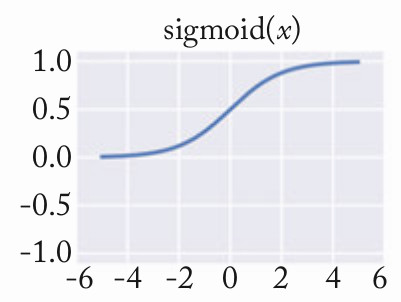
\includegraphics[scale=0.3]{pics/sigmoid2.png}
\end{figure}

\end{scriptsize}
\end{frame}



\begin{frame}{Hyperbolic tangent (tanh)}
\begin{scriptsize}
\begin{itemize}
\item The hyperbolic tangent $\operatorname{tanh}(x) = \frac{e^{2x}-1}{e^{2x}+1}$ activation function is an S-shaped function, transforming the values x into the range$[-1, 1]$.
\end{itemize}

\begin{figure}[htb]
	\centering
	 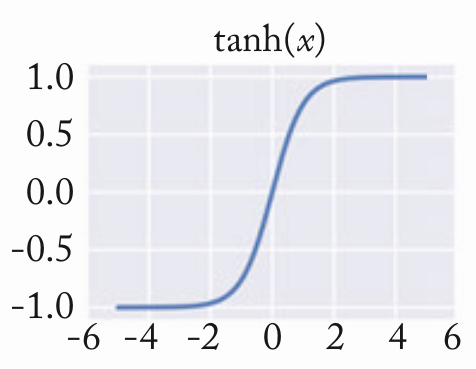
\includegraphics[scale=0.3]{pics/tanh.png}
\end{figure}

\end{scriptsize}
\end{frame}




\begin{frame}{Hard tanh}
\begin{scriptsize}
\begin{itemize}
\item The hard-tanh activation function is an approximation of the tanh function which is faster to compute and to find derivatives thereof:
\end{itemize}

  \[
    \operatorname{hardtanh}(x) = \left\{\begin{array}{lr}
        -1 & x < -1\\
        1 & x > 1\\
        x & \text{otherwise.} 
        \end{array} \right\} 
  \]

\begin{figure}[htb]
	\centering
	 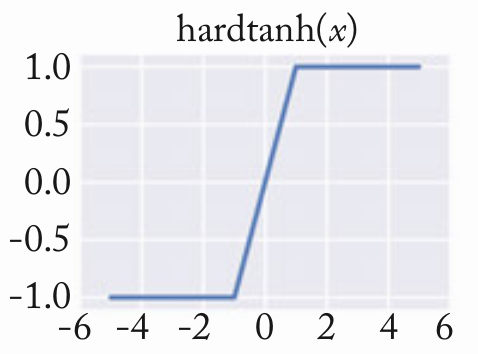
\includegraphics[scale=0.3]{pics/hardtanh.png}
\end{figure}

\end{scriptsize}
\end{frame}



\begin{frame}{ReLU}
\begin{scriptsize}
\begin{itemize}
\item The rectifier activation function \cite{glorot2011deep}, also known as the recti fied linear unit is a very simple activation function.
\item It is easy to work with and was shown many times to produce excellent results.
\item The ReLU unit clips each value $x < 0$ at $0$.
\begin{displaymath}
 \operatorname{ReLU}(x) = \operatorname{max}(0,x)
\end{displaymath}
\begin{figure}[htb]
	\centering
	 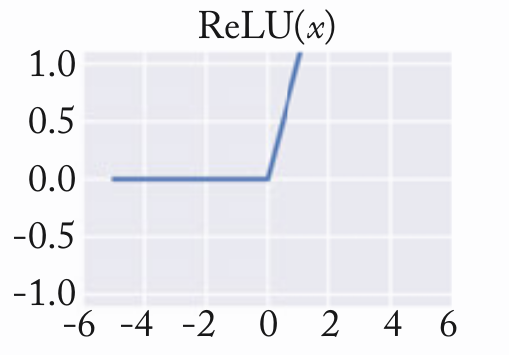
\includegraphics[scale=0.3]{pics/relu.png}
\end{figure}
\item It performs well for many tasks, especially when combined with the dropout regularization technique (to be explained later).
\end{itemize}
\end{scriptsize}
\end{frame}



\begin{frame}{Activation Functions}
\begin{scriptsize}
\begin{itemize}
\item As a rule of thumb, both ReLU and tanh units work well, and significantly outperform the sigmoid.
\item You may want to experiment with both tanh and ReLU activations, as each one may perform better in different settings.
\item The figure from below shows the shapes of the different activations functions, together with the shapes of their derivatives.
\end{itemize}
\begin{figure}[htb]
	\centering
	 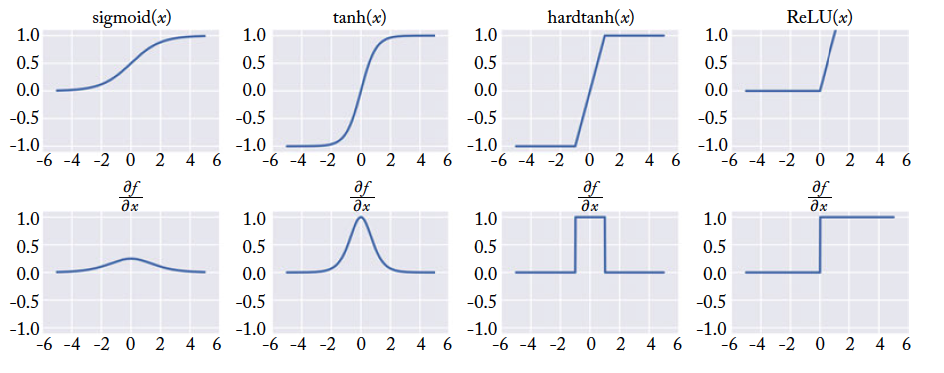
\includegraphics[scale=0.35]{pics/activations.png}
\end{figure}

\footnotetext{Source:\cite{goldberg2017neural}}
\end{scriptsize}
\end{frame}







\begin{frame}{Embedding Layers}
\begin{scriptsize}
\begin{itemize}

\item In NLP the input to the neural network contains symbolic categorical features (e.g., words from a closed vocabulary, character n-grams, POS tags).

\item In linear models we usually represent the input with sparse vectors e.g., as the sum or the concatenation of one-hot encoded vectors (the sum is equivalent to a bag-of words representation). 

\item In neural networks, it is common to associate each possible feature value (i.e., each word in the vocabulary, each POS tag category) with a $d-$dimensional vector for some $d$.

\item These vectors are then considered parameters of the model, and are trained jointly with the other parameters.

\item The mapping from a symbolic feature values such as ``word number 1249'' to $d-$dimensional vectors is performed by an embedding layer (also called a lookup layer ).

\end{itemize}
\end{scriptsize}
\end{frame}


\begin{frame}{Embedding Layers}
\begin{scriptsize}
\begin{itemize}

\item The parameters in an embedding layer are simply a matrix $E \in \mathcal{R}^{|vocab|\times d}$ where each row corresponds to a different word in the vocabulary.

\item The lookup operation is then simply indexing: $v_{1249} = E_{[1249,:]}$.

\item If the symbolic feature is encoded as a one-hot vector $\vec{x}$, the lookup operation can be implemented as a vector-matrix multiplication $\vec{x}E$.

\item The word vectors are often concatenated to each other before being passed on to the next layer.


\item The embeddings matrix $E$ can be initialized with pre-trained word vectors trained from unlabeled documents using specific methods based on the distributional hypothesis such as the ones implemented in Word2Vec (to be discussed later in the course).


\end{itemize}
\end{scriptsize}
\end{frame}




\begin{frame}{Dense Vectors vs. One-hot representations}
\begin{scriptsize}


\begin{itemize}

\item What are the benefits of representing our features as vectors instead of as unique IDs?
\item Should we always represent features as dense vectors? 
\item Let's consider the two kinds of representations.

\item 1) \textbf{One Hot}: each feature is its own dimension. 
\begin{itemize}
\begin{scriptsize}
\item Dimensionality of one-hot vector is same as number of distinct features.
\item Features are completely independent from one another. The feature ``word is `dog' '' is as dissimilar to ``word is `thinking' '' than it is to ``word is `cat' ''.
\end{scriptsize}
\end{itemize}

\item 2) \textbf{Dense}: each feature is a d -dimensional vector. 
\begin{itemize}
\begin{scriptsize}
\item Dimensionality of vector is $d$.
\item Model training will cause similar features to have similar vectors: information is shared between similar features.
\end{scriptsize}
\end{itemize}


\end{itemize}
\end{scriptsize}
\end{frame}


\begin{frame}{Example: Dense Vectors vs. One-hot representations}




\begin{figure}[htb]
	\centering
	 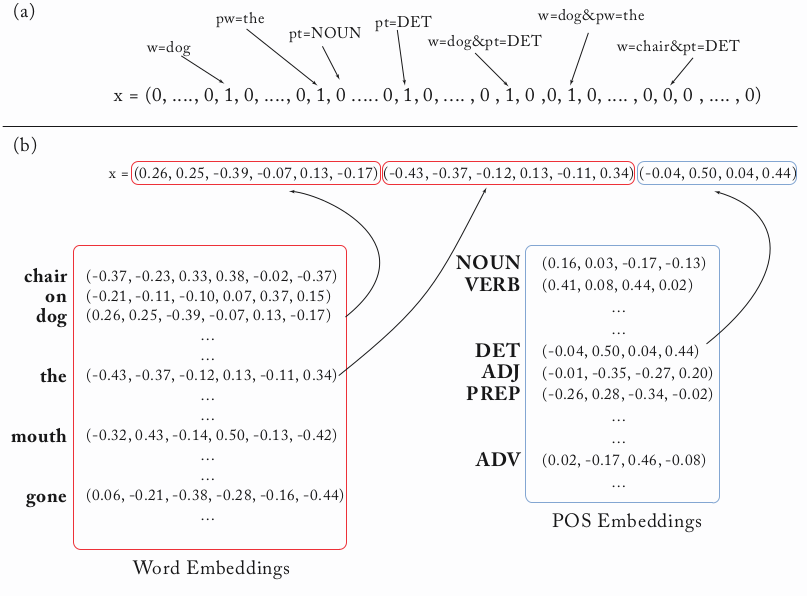
\includegraphics[scale=0.35]{pics/denseonehot.png}
\end{figure}


\end{frame}

\begin{frame}{Example: Dense Vectors vs. One-hot representations}
\begin{scriptsize}


\begin{itemize}

\item Previous figure shows two encodings of the information: current word
is ``dog;'' previous word is ``the;'' previous pos-tag is ``DET.''

\item (a) Sparse feature vector. 
\begin{itemize}
\begin{scriptsize}
\item Each dimension represents a feature. 
\item Feature combinations receive their own dimensions.
\item Feature values are binary. 
\item Dimensionality is very high.
\end{scriptsize}
\end{itemize}

\item (b) Dense, embeddings-based feature vector. 
\begin{itemize}
\begin{scriptsize}
\item Each core feature is represented as a vector.
\item Each feature corresponds to several input vector entries.
\item No explicit encoding of feature combinations.
\item Dimensionality is low.
\item The feature-to-vector mappings come from an embedding table.
\end{scriptsize}
\end{itemize}


\end{itemize}
\end{scriptsize}
\end{frame}




\begin{frame}{Dense Vectors vs. One-hot representations}
\begin{scriptsize}


\begin{itemize}

\item One benefit of using dense and low-dimensional vectors is computational: the majority of neural network toolkits do not play well with very high-dimensional, sparse vectors.
\item However, this is just a technical obstacle, which can be resolved with some engineering effort.

\item The main benefit of the dense representations is in generalization power.

\item If we believe some features may provide similar clues, it is worthwhile to provide a representation that is able to capture these similarities. 

\end{itemize}

\end{scriptsize}
\end{frame}



\begin{frame}{Dense Vectors vs. One-hot representations}
\begin{scriptsize}


\begin{itemize}

\item Let's assume we have observed the word dog many times during
training, but only observed the word cat a handful of times. 

\item If each of the words is associated with its own dimension (one-hot), occurrences of dog will not tell us anything about the occurrences of cat. 

\item However, in the dense vectors representation the learned vector for dog may be similar to the learned vector for cat.

\item This will allow the model to share statistical strength between the two events. 

\item This argument assumes that we saw enough occurrences of the word cat such that its vector will be similar to that of dog.

\item Pre-trained word embeddings (e.g., Word2Vec, Glove) to be discussed later in the course can be used to obtain dense vectors from unanoted text.


\end{itemize}

\end{scriptsize}
\end{frame}

\begin{frame}{Neural Network Training}
\begin{scriptsize}


\begin{itemize}
\item Neural networks are trained in the same way as linear models.

\item The network's output is used to compute a loss fuction $L(\hat{y},y)$ that is minimized across the training examples using gradient descent. 
\item Backpropagation is an efficient technique for evaluating the gradient
of a loss function $L$ for a feed-forward neural network with respect to all its parameters \cite{bishop2006pattern}. \footnote{The following slides on backpropagation are based on \cite{bishop2006pattern}, we adapted the notation to be consistent with \cite{goldberg2017neural}.}
\item Those parameters are: $W^1, \vec{b}^1, \dots, W^m, \vec{b}^m$, for a network of $m$ layers.
\item Recall that superscripts are used to denote layer indexes (not exponentiations).
\item For simplicity, we will assume that $L$ is calculated over a single example.
\item Challenge: in neural networks the number of parameters can be huge and we need an efficient way to calculate the gradients.

\item Idea: apply the derivate chain rule wisely.

\end{itemize}


\end{scriptsize}
\end{frame}


\begin{frame}{Derivative Chain Rule Recap}
\begin{scriptsize}


\begin{itemize}
\item Simple chain rule: let $z = f(y)$, $y = g(x)$, 
\begin{displaymath}
\frac{\partial z}{\partial x} = \frac{\partial z}{\partial y} \times \frac{\partial y}{\partial x}
\end{displaymath}

\item  Example: $z= e^{y}$, $y = 2x$ 

\begin{displaymath}
\frac{\partial z}{\partial x} = \frac{\partial z}{\partial y} \times \frac{\partial y}{\partial x} = e^{y} \times 2 = 2 e^{2x}
\end{displaymath}


\end{itemize}


\begin{figure}[htb]
	\centering
	 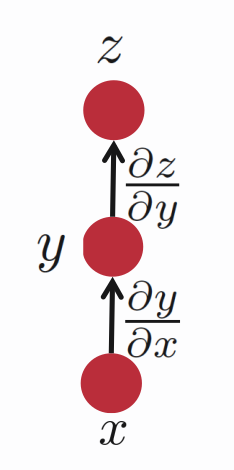
\includegraphics[scale=0.2]{pics/simple_chain_rule.png}
\end{figure}

\footnotetext{Figure taken from:    \url{http://cs224d.stanford.edu/lectures/CS224d-Lecture5.pdf}}

\end{scriptsize}
\end{frame}



\begin{frame}{Derivative Chain Rule Recap}
\begin{scriptsize}


\begin{itemize}
\item Multiple path chain rule: let $z = f(y_1,y_2)$, $y_1 = g_1(x)$, $y_2 =g_2(x)$ 
\begin{displaymath}
\frac{\partial z}{\partial x} = \frac{\partial z}{\partial y_1} \times \frac{\partial y_1}{\partial x} + \frac{\partial z}{\partial y_2} \times \frac{\partial y_2}{\partial x}
\end{displaymath}

\item  Example: $z= e^{y_1 \times y_2}$, $y_1 = 2x$, $y_2 = x^2$ 

\begin{displaymath}
\frac{\partial z}{\partial x} = (e^{y_1 \times y_2}\times y_2) \times 2 + (e^{y_1 \times y_2}\times y_1) \times 2x = e^{2x^3} \times 6x^2
\end{displaymath}


\end{itemize}


\begin{figure}[htb]
	\centering
	 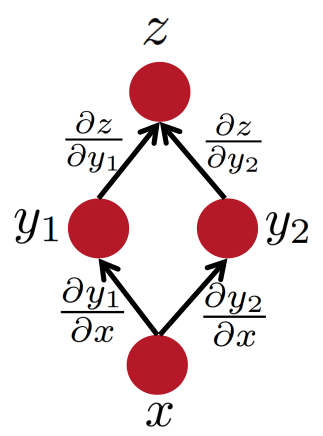
\includegraphics[scale=0.3]{pics/multiple_paths_chain_rule.png}
\end{figure}

\footnotetext{Figure taken from:    \url{http://cs224d.stanford.edu/lectures/CS224d-Lecture5.pdf}}

\end{scriptsize}
\end{frame}



\begin{frame}{Derivative Chain Rule Recap}

The general version of the multiple path chain rule would be:

\begin{displaymath}
 \frac{\partial z}{\partial x} = \sum_{i=1}^n \frac{\partial z}{\partial y_i} \times \frac{\partial y_i}{\partial x} 
\end{displaymath}


\begin{figure}[htb]
	\centering
	 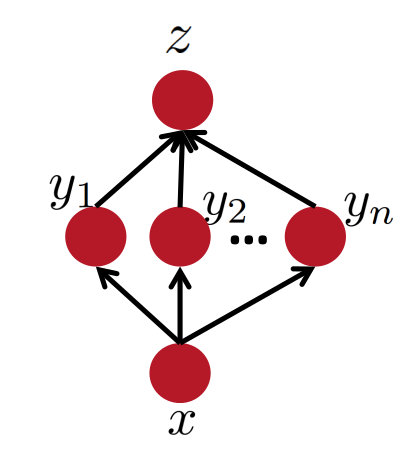
\includegraphics[scale=0.4]{pics/multiple_paths_chain_rule_general.png}
\end{figure}

\footnotetext{Figure taken from:    \url{http://cs224d.stanford.edu/lectures/CS224d-Lecture5.pdf}}

\end{frame}







\begin{frame}{Backpropagation}
\begin{scriptsize}


\begin{itemize}
\item In a general feed-forward network, each unit computes a weighted sum of its inputs in the form:
\begin{equation}
\vec{h}_{[j]}^l = \left(\sum_{i}  W_{[i,j]}^l \times \vec{z}_{[i]}^{(l-1)}\right) + \vec{b}_{[j]}^l 
\label{eq:sum}
\end{equation}

\item The variable $\vec{z}_{[i]}^{(l-1)}$ is an input that sends a connection to unit $\vec{h}_{[j]}^l$, $W_{[i,j]}^l$ is the weight associated with that connection, and $l$ is the layer index.

\item The biases vectors  $\vec{b}_{[j]}$ can be excluded from (eq.\ref{eq:sum}) and included to the weight matrix $W_{[i,j]}^l$ by introducing an extra unit, or input, with activation fixed at +1.

\end{itemize}


\end{scriptsize}
\end{frame}


\begin{frame}{Backpropagation}
\begin{scriptsize}


\begin{itemize}

\item The inputs at layer $l$, $\vec{z}_{[i]}^{(l-1)}$ are the result of applying the activation function $g$ to units from the previous layer:

\begin{equation}
\vec{z}_{[j]}^{l} = g(\vec{h}_{[j]}^{l})
\label{eq:ac}
\end{equation}

\item For the input layer ($l=0$), $\vec{z}$ corresponds to the input vector $\vec{z} = \vec{x}$ 

\begin{equation}
\vec{z}_{[j]}^0 = \vec{x}_{[j]}
\end{equation}

\item For each instance in the training set, we supply the corresponding input vector $\vec{x}$ to the network.
\item Next we calculate the activations of all of the hidden and output units in the network by successive application of (eq.\ref{eq:sum}) and (eq.\ref{eq:ac}). 

\item This process is often called forward propagation because it can be regarded
as a forward flow of information through the network.

\end{itemize}


\end{scriptsize}
\end{frame}


\begin{frame}{Backpropagation}
\begin{scriptsize}


\begin{itemize}

\item Now consider the evaluation of the derivative of $L$ with respect to a weight
$W_{[i,j]}^l$.

\item Assuming that the loss $L$ is calculated over a single example, we can note that $L$ depends on the weight $W_{[i,j]}^l$ only via the summed input $\vec{h}_{[j]}^{l}$.


\item We can therefore apply the chain rule for partial derivatives to give

\begin{equation}
\frac{\partial L}{\partial W_{[i,j]}^l} = \frac{\partial L}{\partial \vec{h}_{[j]}^{l}} \times \frac{\partial \vec{h}_{[j]}^{l}}{\partial W_{[i,j]}^l}
\label{eq:chain}
\end{equation}

\end{itemize}


\end{scriptsize}
\end{frame}



\begin{frame}{Backpropagation}
\begin{scriptsize}


\begin{itemize}


\item We now introduce a useful notation:

\begin{equation}
\vec{\delta}_{[j]}^l \equiv \frac{\partial L}{\partial \vec{h}_{[j]}^l}
\label{eq:delta}
\end{equation}

\item Using (\ref{eq:sum}), we can write
\begin{equation}
\frac{\partial \vec{h}_{[j]}^l}{\partial W_{[i,j]}^l} = \vec{z}_{[i]}^{(l-1)}
\label{eq:part}
\end{equation}

\item Substituting (\ref{eq:delta}) and (\ref{eq:part})  into (\ref{eq:chain}), we then obtain

\begin{equation}
\frac{\partial L}{\partial W_{[i,j]}^l} = \vec{\delta}_{[j]}^l \times \vec{z}_{[i]}^{(l-1)}
\label{eq:deltarule}
\end{equation}

\end{itemize}


\end{scriptsize}
\end{frame}


\begin{frame}{Backpropagation}
\begin{scriptsize}

\begin{itemize}
 \item  Equation (\ref{eq:deltarule}) tells us that the required derivative is obtained simply by multiplying the value of $\vec{\delta}_{[j]}^l$ by the value of $\vec{z}_{[i]}^{(l-1)}$.
 
 \item Thus, in order to evaluate the derivatives, we need only to calculate the value of $\vec{\delta}_{[j]}^l$ for each hidden and output unit in the network, and then apply (\ref{eq:deltarule}).
 
 \item Calculating $\vec{\delta}_{[j]}^m$ for output units ($l=m$), is usually straightforward, since activation units $\vec{h}_{[j]}^m$ are directly observed in the loss expression.
 
 \item The same applies for shallow linear models.
\end{itemize} 
\end{scriptsize}
\end{frame}


\begin{frame}{Backpropagation}
\begin{scriptsize}

\begin{itemize}
 \item To evaluate the $\vec{\delta}_{[j]}^l$ for hidden units, we again make use of the chain rule for partial derivatives:
 
 \begin{equation}
\vec{\delta}_{[j]}^l \equiv \frac{\partial L}{\partial \vec{h}_{[j]}^l} = \sum_{k}\left( \frac{\partial L}{\partial \vec{h}_{[k]}^{l+1}} \times \frac{\partial \vec{h}_{[k]}^{l+1}}{\partial \vec{h}_{[j]}^l}\right)
\label{eq:deltachain}
\end{equation}

\item The sum runs over all units $\vec{h}_{[k]}^{l+1}$ to which unit $\vec{h}_{[j]}^l$ sends connections.

\item We assume that connections go only to consecutive layers in the network (from layer $l$ to layer $(l+1)$).
\item The units $\vec{h}_{[k]}^{l+1}$  could include other hidden units and/or output units.

\item If we now substitute the definition of $\vec{\delta}_{[j]}^l$  given by (eq.\ref{eq:delta}) into (eq.\ref{eq:deltachain}), we get

 \begin{equation}
\vec{\delta}_{[j]}^l \equiv \frac{\partial L}{\partial \vec{h}_{[j]}^l} = \sum_{k}\left( \vec{\delta}_{[k]}^{(l+1)}  \times \frac{\partial \vec{h}_{[k]}^{l+1}}{\partial \vec{h}_{[j]}^l} \right)
\label{eq:delta2}
\end{equation}

\end{itemize}



\end{scriptsize}
\end{frame}



\begin{frame}{Backpropagation}
\begin{scriptsize}

\begin{itemize}
\item Now, for expression $\vec{h}_{[k]}^{l+1}$ we can go to its definition (eq.\ref{eq:sum}): 

\begin{displaymath}
\vec{h}_{[k]}^{(l+1)} = \left( \sum_{i} W_{[i,k]}^{l+1} \times \vec{z}_{[i]}^{l}\right) + \vec{b}_{[k]}^{(l+1)} 
\end{displaymath}

\item Now, we replace (eq.\ref{eq:ac}) $(\vec{z}_{[i]}^{l} = g(\vec{h}_{[i]}^{l}))$  
into previous equation and we obtain:

\begin{displaymath}
\vec{h}_{[k]}^{(l+1)} = \left( \sum_{i}   W_{[i,k]}^{l+1} \times g(\vec{h}_{[i]}^{l})\right)  + \vec{b}_{[k]}^{(l+1)}
\end{displaymath}


\item Now when calculating $\frac{\partial \vec{h}_{[k]}^{l+1}}{\partial \vec{h}_{[j]}^l}$ all the terms in the summation where $i \neq j$ get canceled out.   


\item Hence:

\begin{equation}
\frac{\partial \vec{h}_{[k]}^{l+1}}{\partial \vec{h}_{[j]}^l} =  W_{[j,k]}^{l+1} \times g'(\vec{h}_{[j]}^{l})
\label{eq:partialhh}
\end{equation}


\end{itemize}

\end{scriptsize}
\end{frame}


\begin{frame}{Backpropagation}
\begin{scriptsize}

\begin{itemize}
\item Now, if we substitute (eq.\ref{eq:partialhh}) into (eq.\ref{eq:delta2})


 \begin{equation}
\vec{\delta}_{[j]}^l \equiv \frac{\partial L}{\partial \vec{h}_{[j]}^l} = \sum_{k} \left( \vec{\delta}_{[k]}^{(l+1)}  \times W_{[j,k]}^{l+1} \times g'(\vec{h}_{[j]}^{l}) \right)
\label{eq:delta3}
\end{equation}

\item Since $g'(\vec{h}_{[j]}^{l})$ doesn't depend on $k$ we can obtain the following backpropagation formula:

 \begin{equation}
\vec{\delta}_{[j]}^l = g'(\vec{h}_{[j]}^{l}) \times \sum_{k} \left( \vec{\delta}_{[k]}^{(l+1)}  \times W_{[j,k]}^{l+1}\right)  
\label{eq:delta4}
\end{equation}

\item Which tells us that the value of $\delta$ for a particular hidden unit can be obtained by propagating the $\delta$'s backwards from units higher up in the network. \cite{bishop2006pattern}.

\end{itemize}

\end{scriptsize}
\end{frame}



\begin{frame}{Backpropagation }
\begin{scriptsize}
The backpropagation procedure can  be summarized as follows.
\begin{enumerate}
 \item Apply an input vector $\vec{x}$  to the network and forward propagate through
the network using (eq.\ref{eq:sum}) and (eq.\ref{eq:ac}) to find the activations of all the hidden and output units.
\item Evaluate the $\vec{\delta}_{[j]}^m$ for all the output units (recall that the derivatives involved here are easy to calculate).
\item Backpropagate the $\vec{\delta}_{[k]}^{(l+1)}$ using (eq.\ref{eq:delta4}) to obtain $\vec{\delta}_{[j]}^l$ for each hidden unit in the network. We go from higher to lower layers in the network.
\item Use (eq.\ref{eq:deltarule}) $(\frac{\partial L}{\partial W_{[i,j]}^l} = \vec{\delta}_{[j]}^l \times \vec{z}_{[i]}^{(l-1)})$ to evaluate the required derivatives.
\end{enumerate}


\end{scriptsize}
\end{frame}




\begin{frame}{The Computation Graph Abstraction}
\begin{scriptsize}
\begin{itemize}
\item  One can compute the gradients of the various parameters of a network by hand and implement them in code.

\item This procedure is cumbersome and error prone.

\item For most purposes, it is preferable to use automatic tools for gradient computation \cite{bengio2012practical}.

\item A computation graph is a representation of an arbitrary mathematical computation (e.g., a neural network) as a graph.

\item This abstraction will allow us computing the gradients from any kind of neural network architecture using the backpropagation algorithm. 

\item Previous formulation was restricted to feedforward networks.

\end{itemize}
\end{scriptsize}
\end{frame}


\begin{frame}{The Computation Graph Abstraction}
\begin{scriptsize}
\begin{itemize}
\item A computation graph is a directed acyclic graph (DAG).

\item Nodes correspond to mathematical operations or (bound) variables.

\item Edges correspond to the flow of intermediary values between the nodes.

\item The graph structure defines the order of the computation in terms of the dependencies  between the different components.

\item The graph is a DAG and not a tree, as the result of one operation can be the input of several continuations.

\end{itemize}
\end{scriptsize}
\end{frame}


\begin{frame}{The Computation Graph Abstraction}
\begin{scriptsize}
\begin{itemize}

\item Consider for example a graph for the computation of $(a*b+1)*(a*b+2)$:

\begin{figure}[htb]
	\centering
	 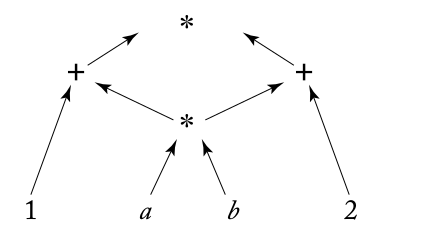
\includegraphics[scale=0.25]{pics/compGraph.png}
\end{figure}

\item The computation of $a*b$ is shared.

\item Since a neural network is essentially a mathematical expression, it can be represented as a computation graph.

\end{itemize}
\end{scriptsize}
\end{frame}




\begin{frame}{The Computation Graph Abstraction}
\begin{scriptsize}

\begin{figure}[htb]
	\centering
	 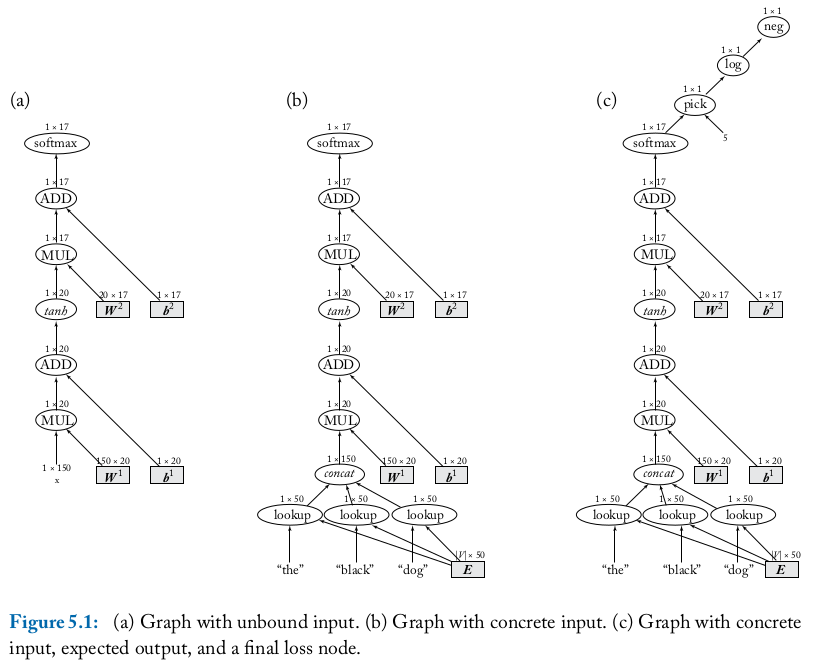
\includegraphics[scale=0.32]{pics/comgraphexample.png}
\end{figure}

\footnotetext{Figure taken from:  \cite{goldberg2017neural}}

\end{scriptsize}
\end{frame}


\begin{frame}{The Computation Graph Abstraction}
\begin{scriptsize}
\begin{itemize}

\item The figure above shows the computation graph for an MLP with one hidden-layer and a softmax output transformation.


\item Oval nodes represent mathematical operations or functions, and shaded rectangle nodes represent parameters (bound variables).

\item Network inputs are treated as constants, and drawn without a surrounding node. 

\item Input and parameter nodes have no incoming arcs, and output nodes have no outgoing arcs. 

\item The output of each node is a matrix, the dimensionality of which is indicated above the node.


\end{itemize}
\end{scriptsize}
\end{frame}


\begin{frame}{The Computation Graph Abstraction}
\begin{scriptsize}
\begin{itemize}

\item This graph is incomplete: without specifying the inputs, we cannot compute an output.

\item Figure 5.1b shows a complete graph for an MLP that takes three words as inputs, and predicts the distribution over part-of-speech tags for the third word. 

\item This graph can be used for prediction, but not for training, as the output is a vector (not a scalar) and the graph does not take into account
the correct answer or the loss term. 

\item Finally, the graph in Figure 5.1c shows the computation graph for a specific training example, in which the inputs are the (embeddings of ) the words ``the,'' ``black,'' ``dog,'' and the expected output is ``NOUN'' (whose index is 5). 

\item The pick node implements an indexing operation, receiving a vector and an index (in this case, 5) and returning  the corresponding entry in the vector.


\end{itemize}
\end{scriptsize}
\end{frame}



\begin{frame}{Forward Computation}
\begin{scriptsize}
\begin{itemize}

\item  The forward pass computes the outputs of the nodes in the graph. \item Since each node's output depends only on itself and on its incoming edges, it is trivial to compute the outputs of all nodes.

\item This is done by traversing the nodes in a topological order and computing the output of each node given the already computed outputs of its predecessors.

\item  More formally, in a graph of $N$ nodes, we associate each node with an index $i$ according to their topological ordering.

\item Let $f_i$ be the function computed by node $i$ (e.g., multiplication,
addition , etc.).



\end{itemize}
\end{scriptsize}
\end{frame}



\begin{frame}{Forward Computation}
\begin{scriptsize}
\begin{itemize}

\item Let $\pi(i)$ be the parent nodes of node $i$ , and $\pi^{-1}(i) = \{j| i \in \pi(j) \}$ the children nodes of node $i$ (these are the arguments of $f_i$).

\item Denote by $v(i)$  the output of node $i$ , that is, the application of $f_i$ to the output values of its arguments $\pi^{-1}(i)$. 

\item For variable and input nodes, $f_i$ is a constant function and $\pi^{-1}(i)$ is empty. 

\item The computation-graph forward pass computes the values $v(i)$ for all $i \in [1,N]$.

 \begin{figure}[htb]
	\centering
	 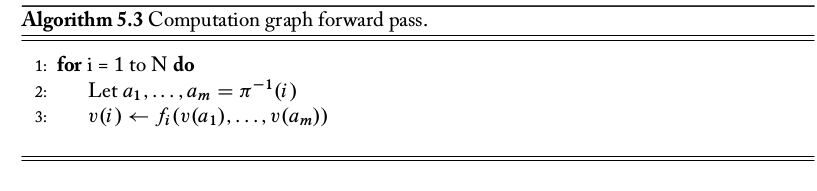
\includegraphics[scale=0.35]{pics/forwardPass.png}
\end{figure}

\end{itemize}
\end{scriptsize}
\end{frame}



\begin{frame}{Backward Computation (Backprop)}
\begin{scriptsize}
\begin{itemize}

\item The backward pass begins by designating a node $N$ with scalar $(1\times1)$ output as a loss-node, and running forward computation up to that node.

\item The backward computation computes the gradients of the parameters with respect to that node's value.


\item Denote by $d(i)$  the quantity $\frac{\partial N}{ \partial i}$.

\item The backpropagation algorithm is used to compute the values $d(i)$  for all nodes $i$.

\item The backward pass fills a table of values $d(1), \dots, d(N)$  as shown in the following algorithm.

 \begin{figure}[htb]
	\centering
	 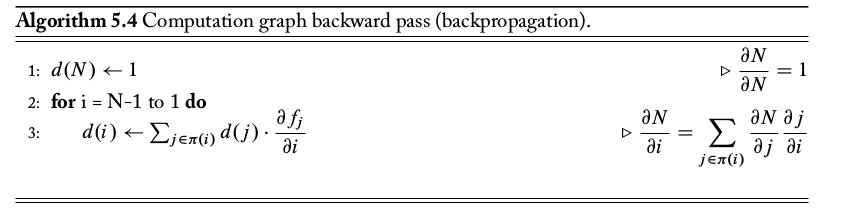
\includegraphics[scale=0.35]{pics/backwardPass.png}
\end{figure}

\end{itemize}
\end{scriptsize}
\end{frame}


\begin{frame}{Backward Computation (Backprop)}
\begin{scriptsize}
\begin{itemize}

\item The backpropagation algorithm is essentially following the chain-rule of differentiation.

\item The quantity  $\frac{\partial f_j}{ \partial i}$ is the partial derivative of $f_j(\pi^{-1}(j))$ w.r.t the argument $i \in \pi^{-1}(j)$.

\item This value depends on the function $f_j$ and the values $v(a_1), \dots, v(a_m)$  (where $a_1, \dots, a_m =  \pi^{-1}(j)$) of its arguments, which were computed in the forward pass.


\item Thus, in order to define a new kind of node, one needs to define two methods: one for calculating the forward value $v(i)$  based on the node's inputs, and the another for calculating  $\frac{\partial f_j}{ \partial i}$ for each $x \in \pi^{-1}(i)$.

\end{itemize}
\end{scriptsize}
\end{frame}


\begin{frame}{Summary of the Computation Graph Abstraction}
\begin{scriptsize}
\begin{itemize}

\item Notice that the above formulation of backpropagation is equivalent to one given earlier in the class.

\item  Te computation graph abstraction allows us to:


\begin{enumerate}
\begin{scriptsize}
 \item Easily construct arbitrary networks.
 \item Evaluate their predictions for given inputs (forward pass)
 
\item Compute gradients for their parameters with respect to arbitrary scalar losses (backward pass or backpropagation).
  
 
\end{scriptsize}
 \end{enumerate}
  
  
\item A nice property of the computation graph abstraction is that it allows computing the gradients for arbitrary networks (e.g., networks with skip-connections, shared weights, special loss functions, etc.)
 
  
\footnotetext{A comprehensive tutorial on the backpropagation algorithm over the computational graph abstraction can be found here: \url{https://colah.github.io/posts/2015-08-Backprop/}.}
 
  
\end{itemize}
\end{scriptsize}
\end{frame}




\begin{frame}{Derivatives of ``non-mathematical'' functions}
\begin{scriptsize}
\begin{itemize}

\item Defining  $\frac{\partial f_j}{ \partial i}$ for mathematical functions such is as $log$ or $+$ is straightforward.

\item It may be challenging to think about the derivative of operations as as pick($\vec{x},5$) that selects the fifth element of a vector.

\item The answer is to think in terms of the contribution to the computation. 

\item After picking the $i$-th element of a vector, only that element participates in the remainder of the computation. 

\item Thus, the gradient of pick($\vec{x},5$) is a vector $\vec{v}$ with the dimensionality of $\vec{x}$ where $\vec{v}_{[5]} =1$ and $\vec{v}_{[i \neq 5]} = 0$.

\item Similarly, for the function $\max(0,x)$  the value of the gradient is $1$ for $x>0$ and $0$ otherwise.

\end{itemize}
\end{scriptsize}
\end{frame}




\begin{frame}{Regularization and Dropout}
\begin{scriptsize}
\begin{itemize}
\item Multi-layer networks can be large and have many parameters, making them especially prone to overfitting.

\item Model regularization is just as important in deep neural networks as it is in linear models, and perhaps even more so.

\item The regularizers discussed for linear models, namely $L_2$ , $L_1$, and the elastic-net, are also relevant for neural networks.

\item Another effective technique for preventing neural networks from overfitting the training data is \textbf{dropout training} \cite{hinton2012improving}.


\end{itemize}
\end{scriptsize}
\end{frame}


\begin{frame}{Regularization and Dropout}
\begin{scriptsize}
\begin{itemize}

\item The dropout method is designed to prevent the network from learning to rely on specific weights.

\item It works by randomly dropping (setting to 0) half of the neurons in the network (or in a specific layer) in each training example in the stochastic-gradient training.


 \begin{figure}[htb]
	\centering
	 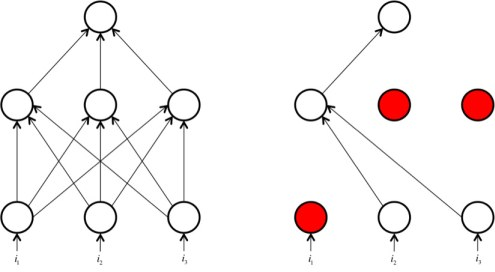
\includegraphics[scale=0.45]{pics/drop-out-in-neural-networks.jpg}
\end{figure}

\footnotetext{Figure taken from:    \url{https://www.kdnuggets.com/wp-content/uploads/drop-out-in-neural-networks.jpg}}

\end{itemize}
\end{scriptsize}
\end{frame}



\begin{frame}{Deep Learning Frameworks}
Several software packages implement the computation-graph model. All these packages support all the essential components (node types) for defining a wide range of neural network architectures.
\begin{scriptsize}
\begin{itemize}
\item TensorFlow (\url{https://www.tensorflow.org/}): an open source software library for numerical computation using data-flow graphs originally developed by the Google Brain Team. 

\item Keras: High-level neural network API that runs on top of Tensorflow as well as other backends (\url{https://keras.io/}). 

\item PyTorch: open source machine learning library for Python, based on Torch, developed by Facebook's artificial-intelligence research group. It supports dynamic graph construction, a different computation graph is created from scratch for each training sample. (\url{https://pytorch.org/})


\end{itemize}
\end{scriptsize}
\end{frame}




\begin{frame}
\frametitle{Questions?}
%\vspace{1.5cm}
\begin{center}\LARGE Thanks for your Attention!\\ \end{center}



\end{frame}

\begin{frame}[allowframebreaks]\scriptsize
\frametitle{References}
\bibliography{bio}
\bibliographystyle{apalike}
%\bibliographystyle{flexbib}
\end{frame}  


%%%%%%%%%%%%%%%%%%%%%%%%%%%

\end{document}
